\section{Related work}


\cpar{Large multimodal models.} A long-standing research goal has been to develop models capable of perceiving the world through multiple modalities, akin to human sensory experience.  Recent progress in vision and language processing has shifted the research focus from smaller, task-specific models toward large, generalist models that can handle diverse inputs \citep{team2023gemini,hurst2024gpt4o}.  Crucially, pre-trained vision and language backbones often require surprisingly little adaptation to enable effective cross-modal communication \citep{tsimpoukelli2021multimodalfrozen,shukor2023epalm,vallaeys2024improveddepalm,merullo2023linearly,koh2023grounding}.  Simply integrating a vision encoder with either an encoder-decoder architecture \citep{shukor2023unival,wang2022ofa,lu2022unified,mizrahi20234m} or a decoder-only LLM has yielded highly capable multimodal systems \citep{laurenccon2024mattersidefics2,alayrac2022flamingo,liu2024improvedllava,wang2024qwen2,xue2024xgenblip3,chen2024internvl,zhu2024minigpt,abdin2024phi3,dai2024nvlm,beyer2024paligemma,moon2024anymal}. This late-fusion approach, where modalities are processed separately before being combined, is now well-understood, with established best practices for training effective models \citep{laurenccon2024obelics,mckinzie2025mm1,zhang2024mm1_5,lin2024vila}.  In contrast, early-fusion models \citep{fuyu8b,team2024chameleon,diao2024unveiling}, which combine modalities at an earlier stage, remain relatively unexplored, with only a limited number of publicly released models \citep{fuyu8b,diao2024unveiling}.  Unlike \citep{diao2024unveiling,team2024chameleon}, our models utilize only a single linear layer and rely exclusively on a next-token prediction loss. Furthermore, we train our models from scratch on all modalities without image tokenization.


\cpar{Native Multimodal Models.} We define native multimodal models as those trained from scratch on all modalities simultaneously \citep{team2023gemini} rather than adapting LLMs to accommodate additional modalities. Due to the high cost of training such models, they remain relatively underexplored, with most relying on late-fusion architectures \citep{kosmoshuang2023language,yu2022coca}. Some multimodal models trained from scratch \citep{aghajanyan2022cm3,team2024chameleon,wang2024emu3} relax this constraint by utilizing pre-trained image tokenizers such as \citep{vqgan,vqvae} to convert images into discrete tokens, integrating them into the text vocabulary. This approach enables models to understand and generate text and images, facilitating a more seamless multimodal learning process.

\cpar{Scaling laws.} Scaling law studies aim to predict how model
performance scales with training compute. Early works
\citep{kaplan2020scaling,hoffmann2022training} found that LLM performance follows
a power-law relationship with compute, enabling the compute-optimal estimation of the number of model parameters and training tokens at scale for a given budget. Similar research has
extended these findings to sparse Mixture of Experts (MoE) models, considering
factors such as sparsity, number of experts, and routing granularity
\citep{krajewski2024scalingmoe,clark2022unifiedscalingmoe,wangscalingmoe}.
Scaling laws have also been observed across various domains, including image
models \citep{fini2024multimodalaimv2}, video models
\citep{rajasegaran2025empirical}, protein LLMs \citep{scalingprotein}, and
imitation learning \citep{pearce2024scaling}. However, few studies have
investigated scaling laws for multimodal models.
Notably,~\citet{aghajanyan2023scalingmm} examined multimodal models that tokenize
modalities into discrete tokens and include multimodal generation. In contrast,
we focus on studying early-fusion models that take raw multimodal inputs and
are trained on interleaved multimodal data.




\cpar{Mixture of experts (MoEs).} Mixture of Experts~\citep{shazeer2017outrageously} enables scaling model capacity by decoupling
model size from per-sample compute. This is done through sparsely
activating a small number of parameters. This approach has led to large
sparse models that rival dense counterparts while being more efficient during
training and inference
\citep{fedus2022switch,sun2024hunyuan,jiang2024mixtral,liu2024deepseekv3,wei2024skywork}.
Many studies have explored improving MoE LLMs across various aspects, such as
load balancing, routing, stability, scaling, and granularity
\citep{lewis2021base,zoph2022st,lepikhin2020gshard}. However, there is limited
research on adopting MoEs for multimodal models, with some work focusing on contrastive
image-text models~\citep{mustafa2022multimodal} and late-fusion multimodal LLMs~\citep{lin2024moe,li2024aria}. Additionally, some studies investigate
predefined expert routing, where certain parameters are reserved to process specific modalities~\cite {bao2021vlmo,chen2024eve,shen2023scaling}. We focus on studying MoEs for native early-fusion models
rather than proposing new architectures.




\begin{figure}[t!]
    \centering
    \captionsetup{type=figure}
    \begin{subfigure}[h]{0.95\linewidth}
    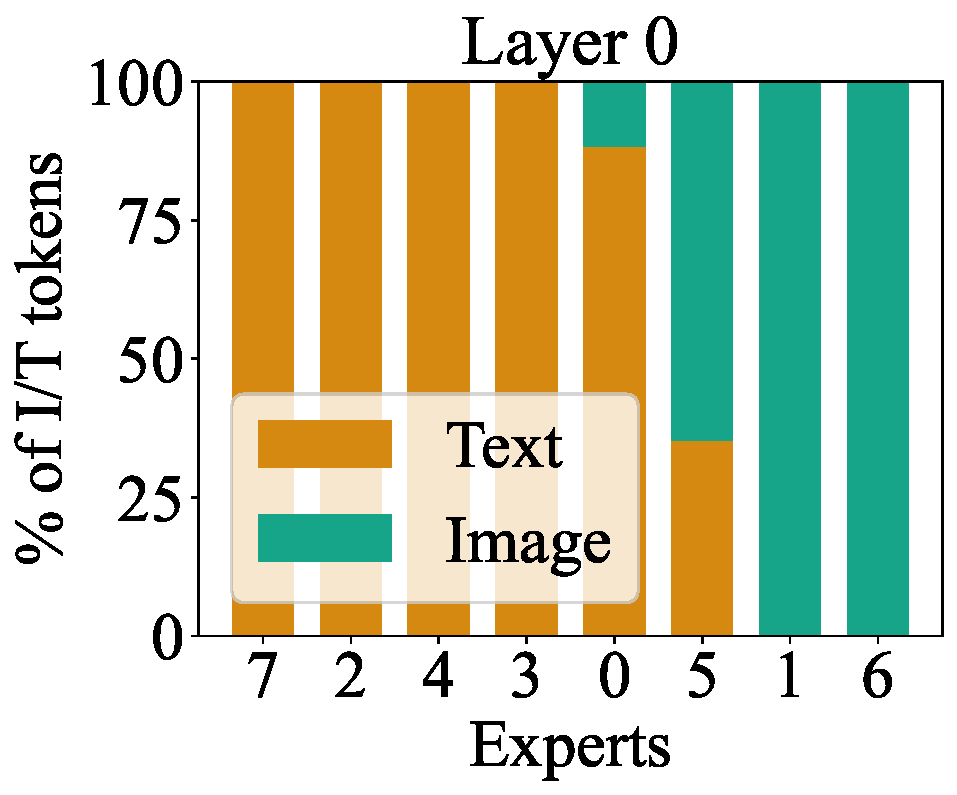
\includegraphics[height=0.27\textwidth]{assets/moes/specialization/sorted/tokens_assignment_obelics_1088_150_0.pdf}
    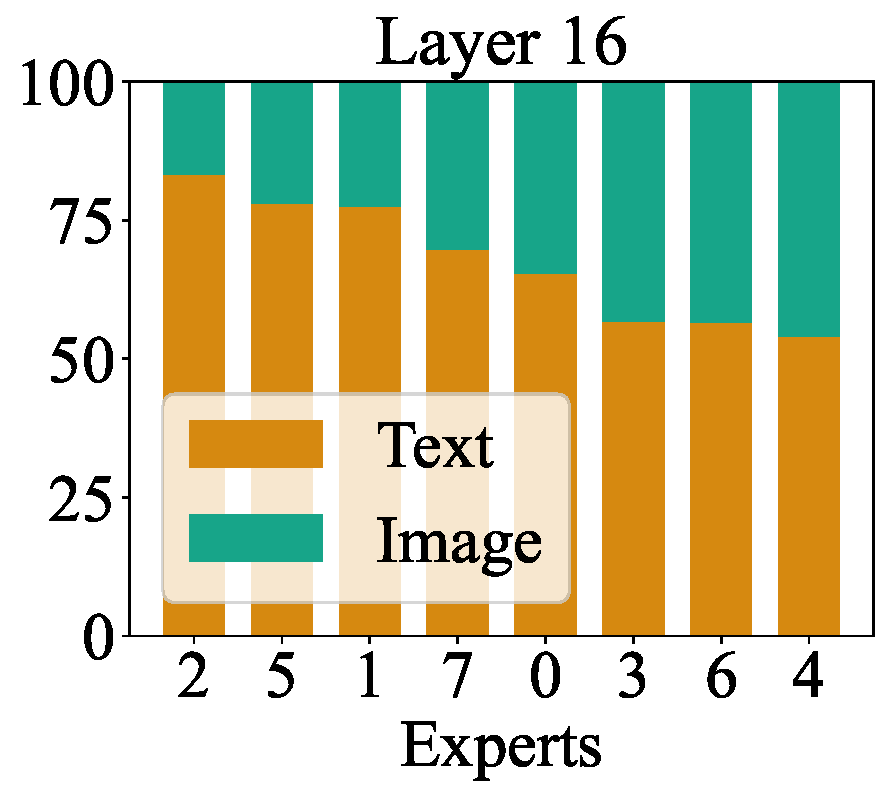
\includegraphics[height=0.27\textwidth]{assets/moes/specialization/sorted/tokens_assignment_obelics_1088_150_16.pdf}
    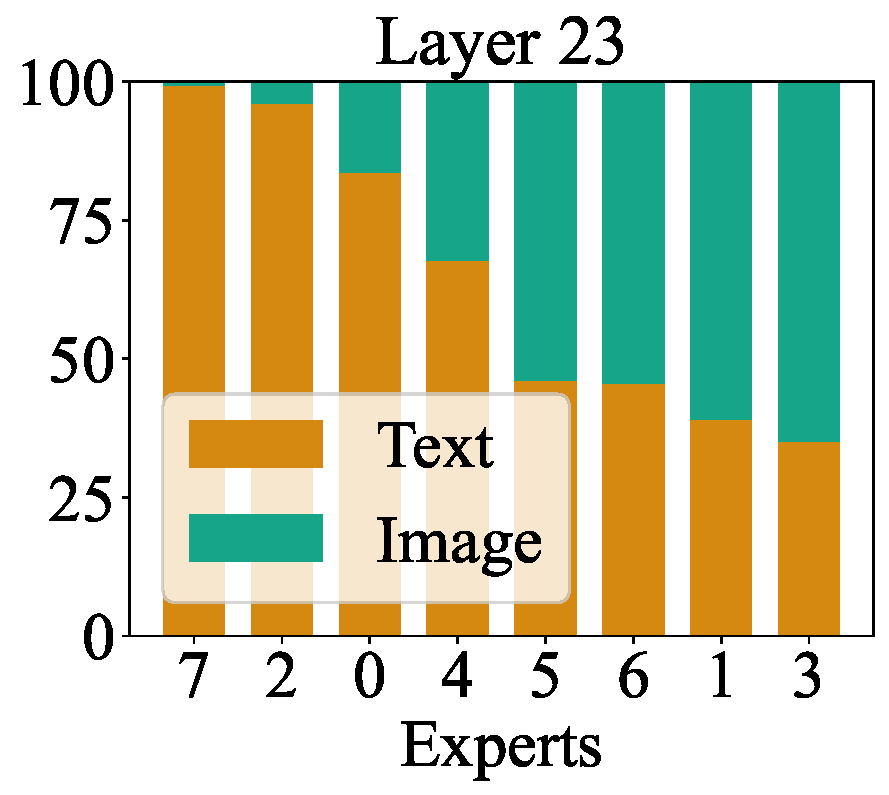
\includegraphics[height=0.27\textwidth]{assets/moes/specialization/sorted/tokens_assignment_obelics_1088_150_23.pdf}
    \end{subfigure}    \caption{\textbf{MoE 特化频率。} 从 Obelics 的交错数据中,路由到每个专家的文本和图像词元的百分比。专家按顺序排列以获得更好的可视化效果。第一层显示了最多的单峰值专家。}
    \label{fig:tokens_assignment}
\end{figure}

